\documentclass[10pt,a4paper,twocolumn]{extarticle}
\usepackage[margin=17mm,top=18mm,bottom=18mm,includeheadfoot]{geometry}
\usepackage[T1]{fontenc}
\usepackage[utf8]{inputenc}
\usepackage{lmodern,microtype,graphicx,booktabs,array,amsmath,amssymb,hyperref,xcolor}
\usepackage[backend=biber,style=authoryear,sorting=nyt,maxbibnames=4]{biblatex}
\addbibresource{ref.bib}
\hypersetup{colorlinks=true,urlcolor=blue!55!black,linkcolor=blue!55!black,citecolor=blue!55!black}
\setlength{\columnsep}{7mm}
\setlength{\parindent}{0pt}
\setlength{\parskip}{3.5pt}
\setlength{\textfloatsep}{7pt}
\setlength{\floatsep}{5pt}
\setlength{\intextsep}{6pt}
\setlength{\abovecaptionskip}{3pt}
\setlength{\belowcaptionskip}{2pt}
\renewcommand{\arraystretch}{1.06}
\usepackage{fancyhdr}
\pagestyle{fancy}\fancyhf{}\fancyhead[C]{\scriptsize COMP-1818 Artificial Intelligence Applications | Francesco Guerriero | 2026/27}\fancyfoot[C]{\thepage}
\setlength{\headheight}{12pt}
\newcommand{\cwtitle}[1]{\title{\vspace{-15mm}\bfseries #1\vspace{-3mm}}}
\newcommand{\cwauthor}[1]{\author{#1}}
\cwtitle{Multi-Objective Evolutionary Feature Selection for Efficient Network Intrusion Detection}
\cwauthor{Francesco Guerriero \\ \small COMP-1818 Individual Report, 2026/27}
\date{17 November 2026}
\begin{document}
\twocolumn[{\centering\LARGE\bfseries Multi-Objective Evolutionary Feature Selection for Efficient Network Intrusion Detection\par\vspace{3pt}\normalsize Francesco Guerriero | COMP-1818 | 17 November 2026\par\vspace{5pt}\hrule\vspace{7pt}}]
\begin{abstract}
Network intrusion detection must balance attack recognition against unnecessary features and false alerts. I compared four evolutionary optimisers (GA, BPSO, continuous-position PSO and NSGA-II) for binary UNSW-NB15 detection, first selecting features alone and then jointly tuning four Random Forest hyperparameters. Each method used five matched random seeds and 300 unique fitness evaluations per seed. Joint PSO achieved the best mean test Macro-F1 (0.8814), using 11.4 of 42 raw predictors (72.9\% reduction), although small-sample statistics and dataset limitations prevent claims of operational superiority.
\end{abstract}
\section{Introduction}
Network intrusion detection systems (NIDS) analyse traffic-flow features to distinguish benign from malicious behaviour. Large predictor sets increase preprocessing, model complexity and computational demand; redundant variables may also worsen generalisation. The engineering challenge is therefore not simply to maximise classification accuracy, but to identify small, reliable feature subsets without obscuring attack detection. False positives matter because unnecessary alerts consume analyst time. The UNSW-NB15 benchmark contains both legitimate and malicious traffic and provides predefined training/testing partitions \parencite{moustafa2015}.

This project asks: Can evolutionary search jointly select informative raw traffic features and tune a Random Forest (RF) to improve binary intrusion detection under a fair computational budget? The outcome is assessed primarily by held-out Macro-F1, which gives equal weight to the benign and attack classes. Balanced accuracy, false-positive rate (FPR), feature count, feature reduction, variability and runtime supply complementary evidence. The goal is comparative research, not an assertion of production-ready live attack detection.

\subsection{Algorithm comparison rationale}
GA, BPSO, PSO and NSGA-II represent deliberately different search behaviours rather than four arbitrary classifiers. GA tests selection, crossover and bit-flip mutation as mechanisms for combining strong feature masks. BPSO tests direct exploration of binary choices using particle memory and social learning. PSO tests whether continuous search dynamics, subsequently converted to binary decisions, provide more effective exploration of a discrete mask space. NSGA-II tests whether explicitly maintaining a Pareto frontier over predictive quality and sparsity yields more compact solutions than a single weighted fitness value. Their comparison exposes trade-offs in accuracy, compression, stochastic stability and optimisation cost \parencite{kennedy1995,kennedy1997,deb2002}.

\subsection{Dataset, protocol and baseline controls}
The official UNSW-NB15 training set contains 175,341 records and the test set 82,332. The target is binary label; id and multiclass attack\_cat are excluded, leaving 42 eligible raw predictors. The official test partition is excluded from feature selection and tuning. Within the official training data, each seed defines a stratified search split (20,000 training / 8,000 validation records). Preprocessing is fitted after selecting raw columns, reducing leakage risk. Selected models are refitted on the full official training partition and assessed against the held-out test set. Five paired seeds (42, 101, 202, 303, 404) permit variation and matched comparisons; baselines include Dummy, Logistic Regression, full-feature RF and XGBoost.

A fair search budget of 300 distinct expensive candidate evaluations per optimiser and seed is enforced with candidate caching. This controls evaluation count rather than wall-clock time: some hyperparameter combinations train much larger forests. The 40 evolutionary runs (four algorithms $\times$ five seeds $\times$ two optimisation modes) amount to 12,000 charged candidate evaluations, excluding full-feature baselines.

\section{Methods}
\subsection{Encoding, objectives and feasibility}
The feature-only chromosome is a 42-bit vector m, with m$_i$ = 1 indicating that raw predictor i is retained. The joint chromosome appends eight bits: four two-bit categorical codes representing RF n\_estimators $\in$ \{40,80,120,200\}, max\_depth $\in$ \{None,12,24,36\}, min\_samples\_leaf $\in$ \{1,2,4,8\} and max\_features $\in$ \{sqrt,log2,0.5,1.0\}. Its valid search space is (2$^{42}$ $-$ 1) $\times$ $4^4$ $\approx$ 1.126 $\times$ 10$^{15}$ combinations. At least one feature bit must be enabled; invalid empty selections are repaired or rejected. Cached duplicates do not consume extra fitness evaluations, but the same mask with different RF settings is counted as a different candidate.

\begin{equation}\label{eq:fitness}F(S,\theta)=\operatorname{MacroF1}_{\mathrm{val}}(S,\theta)-0.05\,\frac{|S|}{42}.\end{equation}
Equation~\eqref{eq:fitness} defines the scalar fitness: $S$ denotes selected raw predictors and 0.05 is the explicit sparsity penalty coefficient. The objective rewards validation detection quality while penalising redundant fields. NSGA-II instead treats validation Macro-F1 (maximise) and |S|/42 (minimise) as two separate objectives, using non-dominated sorting, crowding distance and a validation-only ideal-point compromise. Thus NSGA-II does not simply optimise the same scalar fitness as the other three methods.

\subsection{GA, BPSO and PSO: mechanics}
GA evolves a population of eight binary chromosomes by tournament selection, one-point crossover (probability 0.8) and independent bit mutation (probability 0.05). Elitist survival retains high-fitness candidates; a fresh candidate is injected after stagnation. This can exploit reusable feature combinations but risks population convergence.

BPSO stores an explicitly binary position x $\in$ \{0,1\}$^d$ and real-valued velocity v. Each update combines inertia and attraction to the particle-best and swarm-best masks: v $\leftarrow$ 0.7v + 1.5r$_1$(pbest$-$x) + 1.5r$_2$(gbest$-$x). It then turns velocity into a probability with sigmoid(v), and samples each next bit using a Bernoulli draw. Its coordinates are discrete at every evaluated position.

PSO in this implementation instead keeps continuous positions x $\in$ [0,1]$^d$, updates v using the same inertia/cognitive/social coefficients (0.7, 1.5, 1.5), clips x+v into [0,1] and binarises only for model evaluation using x $\geq$ 0.5. Its personal/global bests remain continuous positions. Consequently, BPSO is probabilistic bit sampling driven by velocity, whereas PSO is continuous movement plus deterministic thresholding. This distinction matters because their exploration and duplicate-mask behaviour differ despite similar parameter names. Both use eight particles and stagnation recovery.

NSGA-II is intentionally different: its non-dominated sorting distinguishes solutions that no other candidate beats simultaneously in validation F1 and feature count, while crowding-distance selection preserves diversity along the trade-off. The exported single compromise minimises validation-only ideal-point distance; the complete seed-specific Pareto sets are retained for further analysis \parencite{deb2002}.

\subsection{Hybrid implementation and reproducibility}
The wrapper hybridises nature-inspired search with supervised RF fitting: a candidate mask/parameter set is evaluated using training-derived validation Macro-F1, then the selected RF is refitted and tested. Advanced controls include fixed seeds, a 300-unique-evaluation budget, duplicate caching, nonempty-mask repair, multi-objective Pareto archive, final-model export, dataset/source hashes in manifests, and a passive Windows IDS prototype with a React interface. The prototype replays compatible feature rows; live socket telemetry does not supply every UNSW-NB15 feature and must not be equated with validated live-flow classification.

A real implementation defect was discovered: the joint-mode command-line argument was initially not forwarded to the evaluator. That run produced feature-only results and was invalidated. The corrected 16 November experiment records nonempty selected RF hyperparameters in all 20 joint runs. A CLI-level regression test now guards the forwarding path; 21 Python tests and dataset-free Windows CI passed. This is substantive debugging evidence, not merely a proposed feature.

\section{Experiments and Results}
Table~\ref{tab:results} reports five-seed averages from the corrected full experiment. All methods received 300 unique candidate evaluations per seed. Joint PSO attained the highest mean test Macro-F1 and lowest mean FPR among the four evolutionary searches. NSGA-II achieved the most aggressive compression but poorer detection quality.

\begin{table}[ht]\centering\scriptsize
\resizebox{\columnwidth}{!}{\begin{tabular}{lrrrrr}\toprule
Method & Feature F1 $\pm$ SD & Joint F1 $\pm$ SD & Joint features & Reduction & Joint FPR \\ \midrule
GA & $.8612\pm.0082$ & $.8789\pm.0185$ & 9.8 & 76.67\% & .2244 \\
BPSO & $.8594\pm.0107$ & $.8772\pm.0128$ & 12.6 & 70.00\% & .2304 \\
PSO & $.8643\pm.0129$ & $\mathbf{.8814\pm.0081}$ & 11.4 & 72.86\% & .2197 \\
NSGA-II & $.8397\pm.0390$ & $.8439\pm.0247$ & 6.0 & 85.71\% & .2676 \\
\bottomrule\end{tabular}}
\caption{Held-out UNSW-NB15 binary-classification results, averaged over the same five random seeds (42, 101, 202, 303, 404). Macro-F1 values are mean $\pm$ sample standard deviation; joint selected raw-feature count, reduction relative to 42 predictors, and false-positive rate (FPR) are five-seed means. Each algorithm received 300 unique expensive candidate evaluations per seed in both modes; higher Macro-F1 and lower FPR are preferred.}\label{tab:results}\end{table}
\begin{figure}[ht]\centering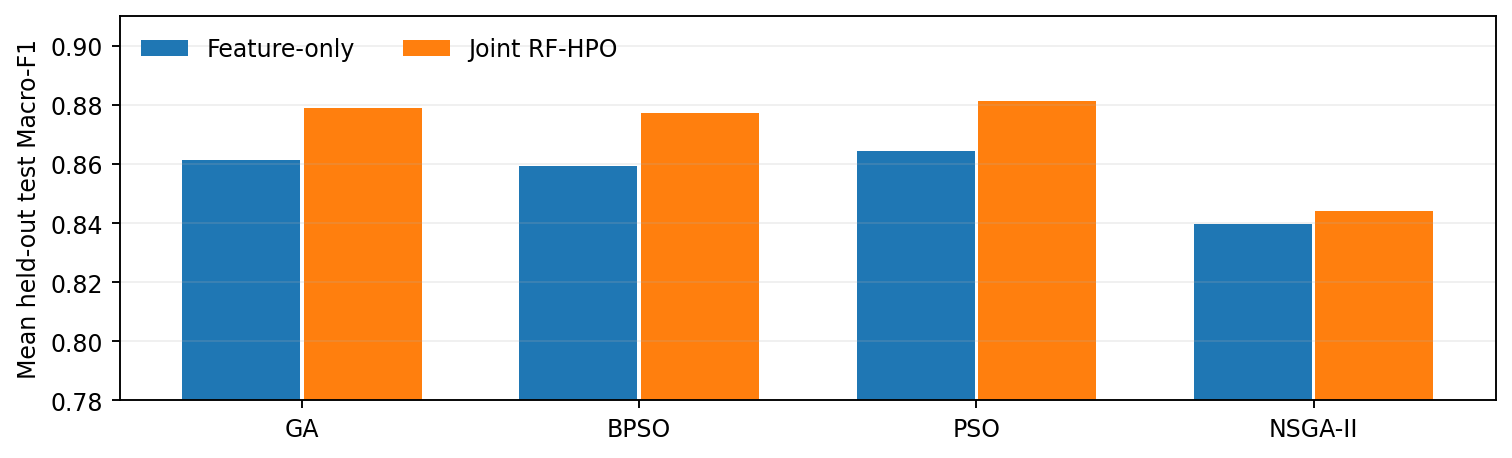
\includegraphics[width=\columnwidth]{figures/figure1.png}\caption{Comparison of feature-only selection and joint feature-selection/Random Forest hyperparameter optimisation (RF-HPO). Bar heights give mean Macro-F1 on the held-out official UNSW-NB15 test partition over five matched seeds per algorithm. The vertical axis is truncated at 0.78 to display differences; consult Table~\ref{tab:results} for exact scores and standard deviations. Generated from the published feature-only and corrected-joint summary CSVs using Matplotlib.}\label{fig:performance}\end{figure}
\begin{figure}[ht]\centering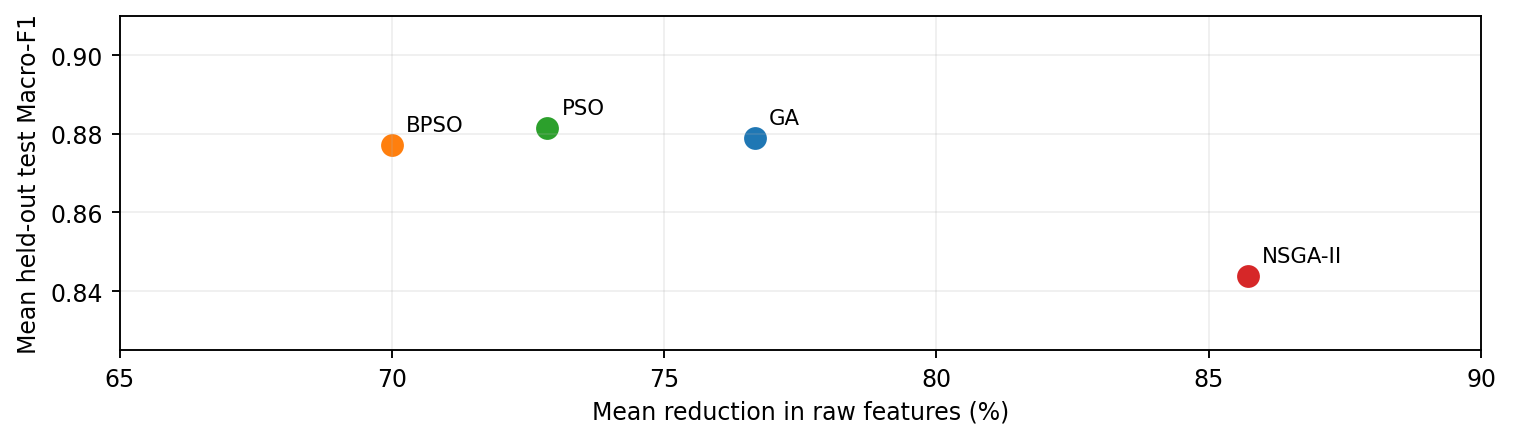
\includegraphics[width=\columnwidth]{figures/figure2.png}\caption{Accuracy--dimensionality trade-off for the corrected joint RF-HPO experiment. Each point is one algorithm, positioned by its five-seed mean held-out test Macro-F1 (vertical) and mean percentage reduction from 42 raw predictors (horizontal). Up and right indicate higher accuracy and greater compression, respectively; there is no single best method on both axes. Generated using Matplotlib from the corrected joint summary CSV.}\label{fig:tradeoff}\end{figure}
Figure~\ref{fig:performance} visualises the gains in Table~\ref{tab:results}; Figure~\ref{fig:tradeoff} shows why Macro-F1 and feature reduction must be evaluated jointly. In particular, PSO attains the highest mean test Macro-F1, whereas NSGA-II attains the largest dimensionality reduction.

\subsection{Figure generation and report traceability}
The visual evidence is reproducible rather than manually redrawn. The accompanying \texttt{figures/generate\_figures.py} reads the saved feature-only and corrected joint summary CSVs, plots five-seed means with Matplotlib, and exports Figures~\ref{fig:performance} and~\ref{fig:tradeoff} as PNG files using \texttt{plt.savefig()}. Figure~\ref{fig:performance} compares held-out Macro-F1 between the two optimisation protocols; Figure~\ref{fig:tradeoff} relates predictive quality to the percentage of raw features removed. Neither plot uses synthetic demonstration outputs or the superseded joint-labelled run. Each caption identifies the metric, experimental source and interpretation of the axes, so it remains understandable independently of the surrounding prose.

Tables~\ref{tab:results} and~\ref{tab:paired} are typeset directly with LaTeX \texttt{tabular} and \texttt{booktabs}, not inserted as images. The former reports performance and dimensionality; the latter reports matched-seed effect estimates and uncertainty. Equation~\eqref{eq:fitness} is written with the \texttt{equation} environment so its notation is selectable and consistently numbered. Numbered labels and LaTeX cross-references link each display to its interpretation in the report. The provided CSV files and plotting script allow the figures to be regenerated and checked against the published results.


The comparison in Figure~\ref{fig:performance} is intentionally aggregated at the method level. Means summarise the five independent seeds, but they conceal seed-to-seed dispersion; Table~\ref{tab:results} therefore also reports standard deviations. The separate trade-off display in Figure~\ref{fig:tradeoff} does not establish a universally optimal feature set. Therefore the graphs complement, rather than replace, the run-level statistics.

Reproducing a figure is distinct from reproducing a complete training run. The script transforms versioned summary records into visual output; it does not refit RF models or repeat evolutionary search. A stronger replication would first obtain the official data partitions, verify their SHA-256 checksums against the run manifest, execute the recorded search configuration, and compare new per-seed outputs with the archived CSVs. Plot generation alone does not revalidate benchmark accuracy.
\subsection{Matched-seed statistical comparison}
\begin{table}[ht]\centering\scriptsize
\resizebox{\columnwidth}{!}{\begin{tabular}{lrrrr}\toprule
Algorithm & Paired gain & 95\% $t$ CI & Paired $t$ $p$ & Wilcoxon $p$ \\ \midrule
GA & +.01771 & [$-.00521$,$+.04063$] & .0985 & .1250 \\
BPSO & +.01776 & [$-.00691$,$+.04244$] & .1163 & .0625 \\
PSO & +.01709 & [$+.00666$,$+.02752$] & .0104 & .0625 \\
NSGA-II & +.00420 & [$-.05652$,$+.06493$] & .8569 & .8125 \\
\bottomrule\end{tabular}}
\caption{Within-algorithm paired differences in held-out Macro-F1, calculated as joint minus feature-only over five matched seeds. Reported quantities are mean paired improvement, the two-sided 95\% paired $t$ interval, and unadjusted paired $t$-test and exact two-sided Wilcoxon signed-rank $p$-values. With only five seeds and four comparisons, these are exploratory rather than confirmatory significance tests.}\label{tab:paired}\end{table}
Table~\ref{tab:paired} reports the paired-seed uncertainty. Full-feature baselines yielded Macro-F1 0.3551 (Dummy), 0.8292 (Logistic Regression), 0.8641 $\pm$ 0.0004 (RF) and 0.8668 $\pm$ 0.0008 (XGBoost). Joint PSO exceeded the XGBoost mean by 0.0146 in this benchmark while retaining only 11.4/42 predictors. These cross-family differences are descriptive; they are not inferential proof of superiority under different training protocols.

The feature-only and corrected joint experiments were evaluated using matched algorithm/seed pairs rather than selecting the single best test run. Joint GA reduced the mean selected features from 10.2 to 9.8, whereas joint PSO used 11.4 versus 11.2; this illustrates that joint tuning may improve detection without uniformly reducing model inputs. PSO reduced mean FPR from 0.2563 to 0.2197 (3.66 percentage points). These are empirical benchmark differences, not guaranteed real-world alert reductions.

\section{Discussion and Conclusion}
\subsection{Comparison with previous work}
Unlike classic feature-selection-only wrappers, the corrected study searches feature subsets and RF hyperparameters simultaneously; unlike a purely scalar search, NSGA-II exposes a two-objective sparsity--accuracy frontier. Earlier local EvoNIDS summary figures and the invalid joint-labelled run are not substituted for the corrected study: the former can differ in code/configuration and the latter accidentally ran feature-only optimisation. Relative to the matched November 2026 feature-only experiment, mean test Macro-F1 improved by +0.01771 (GA), +0.01776 (BPSO), +0.01709 (PSO) and +0.00420 (NSGA-II).

For PSO the paired gain was +0.01709 (95\% t confidence interval +0.00666 to +0.02752; paired t-test p = 0.0104). All five PSO seeds improved, but the exact two-sided Wilcoxon p-value was 0.0625. Four simultaneous algorithm comparisons and only five stochastic repetitions limit inferential confidence. GA improved in four seeds, BPSO in five and NSGA-II in three; their respective paired t-test p-values were 0.0985, 0.1163 and 0.8569. Reporting both effect sizes and uncertainty avoids overstating significance.

The comparisons are deliberately paired because stochastic runs from the same seed correspond to matched evaluation settings. For NSGA-II the changes are particularly unstable: a mean F1 gain of only 0.0042 accompanies a 95\% t interval spanning $-$0.0565 to +0.0649. The exact Wilcoxon p-values for PSO and BPSO are 0.0625 despite improvements in every matched seed, reflecting the coarse resolution of exact two-sided tests with just five pairs. Furthermore, the four tests are not independent evidence of four separate guaranteed improvements; multiple-testing correction and replication are necessary.

\subsection{Limitations and future investigation}
The primary limitation is external validity: an offline binary UNSW-NB15 benchmark does not demonstrate robust detection of novel attacks, temporal drift or live operational traffic. The Windows prototype only observes passive socket information, not a complete UNSW flow record. Secondary limitations are the relatively small search-training sample, five seeds, the preset 0.05 feature penalty, restricted categorical RF search grid, limited RF/model-family comparisons and the gap between equal evaluation counts and unequal fit times. In addition, repeated test-set comparisons could encourage post-hoc model selection; a deployment candidate should be selected by validation criteria and confirmed on an additional untouched dataset.

A practical next stage would evaluate attack-wise recall and false-alert rates under realistic class prevalence; measure fitting/inference cost and feature acquisition overhead; conduct penalty and budget ablations (e.g., 100/300/600 evaluations); add an external or temporally separated test set; and assess calibration and feature-set stability. NSGA-II should be judged using complete Pareto quality and deployment constraints, not only the selected compromise point. These improvements would distinguish a promising academic benchmark from defensible operational security.

Equal search evaluations do not imply equal training cost because RF configurations vary from 40 to 200 trees. The manifests record source and dataset hashes; CI verifies the synthetic pipeline and statistics, not the complete dataset-based training runs.


The distinction between false-positive rate and feature reduction is also important when assessing deployment value. Lower FPR on the held-out benchmark means fewer benign records are misclassified \emph{within that dataset}, not necessarily fewer alerts per hour in a different network. Feature reduction measures input dimensionality, not proportional savings in acquisition or inference time: some retained flow statistics still require expensive aggregation. A deployment evaluation should therefore report measured latency, throughput and the cost of obtaining each selected field, alongside Macro-F1 and FPR, before claiming operational efficiency.

\subsection{Overall conclusion}
Joint evolutionary feature selection and RF tuning delivered a useful accuracy--sparsity trade-off. Under the controlled five-seed, equal-evaluation protocol, PSO was the strongest average option (Macro-F1 0.8814; 72.86\% feature reduction; mean FPR 0.2197), whereas NSGA-II prioritised compression (85.71\% reduction). The contribution is a comparative, auditable optimisation workflow with explicit treatment of a corrected experimental defect---not a claim of universal algorithm dominance. The next requirement is out-of-distribution validation and real flow-feature extraction before deployment.

\subsection{Generative-AI use and verification reflection}
Generative AI helped explain methods, review code, organise the report and improve wording. The results come from executed Python experiments and saved CSV files. I corrected and reran an invalid joint-optimisation experiment, verified the statistics and checked the report against the recorded outputs. I remain responsible for the analysis and conclusions.

\clearpage
\onecolumn
\section*{References and reproducibility}
\nocite{*}
\printbibliography[heading=none]
\vspace{5pt}
\noindent\textbf{Repository:} \url{https://github.com/FrancescoGuerriero/COMP1818_EvoNIDS_with_React}\\
\textbf{Dataset:} \url{https://research.unsw.edu.au/projects/unsw-nb15-dataset}\\
\textbf{Corrected joint experiment:} \url{https://github.com/FrancescoGuerriero/COMP1818_EvoNIDS_with_React/tree/main/COMP1818_EvoNIDS_Submission/results/protocol_runs/20261116T151402Z_full_joint}\\
\textbf{Paired analysis:} \url{https://github.com/FrancescoGuerriero/COMP1818_EvoNIDS_with_React/blob/main/COMP1818_EvoNIDS_Submission/results/statistical_analysis/paired_joint_comparison.csv}\\
\footnotesize Recorded results are distinguished from synthetic CI tests; the earlier mislabelled joint run is excluded.
\end{document}
